\documentclass[11pt,a4paper]{article}
\usepackage[T1]{fontenc}
\usepackage[utf8]{inputenc}
\usepackage{lmodern}
\usepackage{geometry}
\usepackage{amsmath}
\usepackage{amssymb}
\usepackage{graphicx}
\geometry{margin=1in}
\graphicspath{{./figures/}{../../data/figures/}}

\title{02225 DRTS Mini-Project 1\\Report on Deadline Monotonic and Earliest Deadline First Scheduling}
\author{Group: <replace with names and student IDs>}
\date{\today}

\begin{document}
\maketitle

\section{Introduction \& Theory}

\subsection{Project Goals}
The project develops analytical tools for worst-case response-time (WCRT) analysis of periodic real-time tasks under Deadline Monotonic (DM) and Earliest Deadline First (EDF) scheduling. The implementation is validated against a discrete-event simulator, and the two scheduling policies are compared with respect to schedulability, WCRTs, preemptions, and deadline misses. The main implementation path is the scheduler analysis tool in \texttt{scheduler\_analysis.py}.

\subsection{Scheduling Model and Notation}
The task model is a periodic task set
\begin{equation}
\Gamma = \{\tau_1, \tau_2, \ldots, \tau_n\},
\end{equation}
where each task \(\tau_i\) is characterised by the tuple \((C_i, D_i, T_i)\) analytically and by \((\mathrm{BCET}_i, C_i, D_i, T_i)\) in simulation. Table~\ref{tab:notation} defines the notation used throughout the report.

\begin{table}[h]
\centering
\small
\begin{tabular}{|l|p{0.68\linewidth}|}
\hline
Symbol & Meaning \\
\hline
\(C_i\) & Worst-case execution time (WCET) of task \(\tau_i\) \\
\hline
\(D_i\) & Relative deadline, with \(C_i \leq D_i \leq T_i\) \\
\hline
\(T_i\) & Period of \(\tau_i\) \\
\hline
\(U_i = C_i/T_i\) & Utilisation of task \(\tau_i\) \\
\hline
\(U = \sum_{i=1}^{n} U_i\) & Total processor utilisation \\
\hline
\(H = \mathrm{lcm}(T_1,\ldots,T_n)\) & Hyperperiod \\
\hline
\(r_{i,k} = (k-1)T_i\) & Release time of the \(k\)-th job of \(\tau_i\) \\
\hline
\(d_{i,k} = r_{i,k} + D_i\) & Absolute deadline of the \(k\)-th job \\
\hline
\(f_{i,k}\) & Finish time of the \(k\)-th job \\
\hline
\(R_{i,k} = f_{i,k} - r_{i,k}\) & Response time of the \(k\)-th job \\
\hline
\(\mathrm{WCRT}_i = \max_k R_{i,k}\) & Worst-case response time of task \(\tau_i\) \\
\hline
\end{tabular}
\caption{Essential notation.}
\label{tab:notation}
\end{table}

\subsection{Assumptions}
The implementation and all analytical results are based on the following assumptions:
\begin{enumerate}
  \item Synchronous release: all tasks release their first job at \(t=0\).
  \item Constrained deadlines: \(D_i \leq T_i\) for all tasks.
  \item Fixed WCETs in analysis: the analytical tools assume each job executes for exactly \(C_i\).
  \item Independent tasks: no precedence constraints or shared resources are modelled.
  \item Fully preemptive single-processor scheduling.
  \item Zero kernel and dispatch overhead.
  \item In simulation only, execution times are sampled from \([\mathrm{BCET}_i, C_i]\).
\end{enumerate}

\subsection{Scheduling Algorithms}

\subsubsection{Deadline Monotonic}
Deadline Monotonic assigns a fixed priority inversely proportional to relative deadline \cite{LW82,buttazzo2024}:
\begin{equation}
D_i < D_j \implies \mathrm{priority}(\tau_i) > \mathrm{priority}(\tau_j).
\label{eq:dm-priority}
\end{equation}
DM is optimal among fixed-priority assignments \cite{buttazzo2024}. When \(D_i=T_i\) for all tasks, DM reduces to Rate Monotonic (RM). The classical Liu--Layland sufficient bound is
\begin{equation}
U \leq n\left(2^{1/n} - 1\right),
\label{eq:ll-bound}
\end{equation}
which converges to \(\ln 2 \approx 0.69\) as \(n \to \infty\) \cite{LL73}. A tighter sufficient test is the hyperbolic bound \cite{Bini2001}:
\begin{equation}
\prod_{i=1}^{n}(U_i + 1) \leq 2.
\label{eq:hyperbolic}
\end{equation}
The implementation uses exact response-time analysis rather than only sufficient tests.

\subsubsection{Earliest Deadline First}
EDF is a dynamic-priority algorithm that always executes the ready job with the earliest absolute deadline \cite{LL73}. For implicit-deadline systems, schedulability is characterised exactly by
\begin{equation}
\sum_{i=1}^{n} \frac{C_i}{T_i} \leq 1.
\label{eq:edf-util}
\end{equation}
For constrained-deadline systems, the exact schedulability test is the processor-demand criterion (PDC) \cite{Baruah1990,buttazzo2024}. The demand-bound function is
\begin{equation}
\mathrm{dbf}(t) = \sum_{i=1}^{n} \left\lfloor \frac{t + T_i - D_i}{T_i} \right\rfloor C_i,
\label{eq:dbf}
\end{equation}
and the task set is EDF schedulable iff
\begin{equation}
\forall t \in \mathcal{D}: \quad \mathrm{dbf}(t) \leq t,
\label{eq:pdc}
\end{equation}
where \(\mathcal{D}\) contains the relevant absolute deadlines up to
\begin{equation}
L^* = \frac{\sum_{i=1}^{n} U_i(T_i - D_i)}{1-U}.
\label{eq:lstar}
\end{equation}
Only deadlines up to \(\min(H,\max(D_{\max},L^*))\) need to be checked \cite{buttazzo2024}.

\subsubsection{Key Comparison Points}
The comparison section uses the following theory results. Cervin shows that under permanent overload, EDF degrades by effective period rescaling whereas low-priority tasks under RM/DM can be starved in the stationary regime \cite{Cervin2003}. Cervin also states that the maximum input--output latency under EDF is shorter than or equal to that under DM/RM for comparable periodic task chains \cite{Cervin2003}. Buttazzo reports that RM preemptions tend to increase approximately linearly with load, while EDF preemptions may flatten or decrease at high utilisation because delayed jobs skip some otherwise possible preemption points \cite{Buttazzo2005}.

\section{Implementation}

\subsection{Tool Overview}
Two software tools were implemented in Python. The analytical tool, centred on \texttt{scheduler\_analysis.py}, computes exact DM WCRTs via response-time analysis, checks EDF schedulability with the PDC, and computes exact EDF WCRTs by deterministic schedule construction when the hyperperiod remains tractable. The simulation tool reuses the same task model and performs preemptive WCET and stochastic executions using \texttt{heapq}, \texttt{math.lcm}, \texttt{pandas}, and \texttt{numpy}. The main commands are:

\begin{verbatim}
python3 -m py_compile scheduler_analysis.py test_all_tasksets.py
python3 test_all_tasksets.py
python3 scheduler_analysis.py
\end{verbatim}

\subsection{DM Response-Time Analysis}
The exact DM WCRT for task \(\tau_i\) is obtained by the fixed-point equation \cite{Audsley1993,buttazzo2024}
\begin{equation}
R_i = C_i + \sum_{j:\,D_j < D_i} \left\lceil \frac{R_i}{T_j} \right\rceil C_j.
\tag{RTA}
\label{eq:rta}
\end{equation}
It is solved iteratively from
\begin{equation}
R_i^{(0)} = C_i
\label{eq:rta-init}
\end{equation}
and
\begin{equation}
R_i^{(s)} = C_i + \sum_{j:\,D_j < D_i} \left\lceil \frac{R_i^{(s-1)}}{T_j} \right\rceil C_j.
\label{eq:rta-iter}
\end{equation}
The implementation stops when the sequence converges or when \(R_i^{(s)} > D_i\), in which case the task set is infeasible under DM.

\begin{verbatim}
Algorithm RTA(Gamma)
  sort tasks by increasing D_i, breaking ties by task index
  for each task tau_i in DM order:
      R <- C_i
      repeat
          R_old <- R
          I <- sum over higher-priority tasks of ceil(R_old / T_j) * C_j
          R <- C_i + I
          if R > D_i: return infeasible
      until R = R_old
      WCRT_i <- R
  return schedulable, {WCRT_i}
\end{verbatim}

The improved initial guess suggested by Buttazzo is
\begin{equation}
R_i^{(0)} = \max\left(R_{i-1}+C_i, \; \frac{C_i}{1-\sum_{j=1}^{i-1} U_j}\right),
\label{eq:rta-improved}
\end{equation}
but the present code keeps the simpler initialisation \(R_i^{(0)}=C_i\) for clarity.

\subsection{EDF Exact WCRT by Hyperperiod Simulation}
For synchronous periodic tasks with fixed WCETs, the EDF schedule is deterministic over one hyperperiod. The implementation therefore generates all jobs released in \([0,H)\), executes them with WCET, and records
\begin{equation}
R_{i,k} = f_{i,k} - r_{i,k}, \qquad \mathrm{WCRT}_i = \max_k R_{i,k}.
\label{eq:edf-wcrt}
\end{equation}
The code uses a ready queue ordered by \((d_{i,k}, i, k)\), i.e., ties are broken by lower task index and then job index, matching the analytical and simulation models. The exact analysis is guarded by \texttt{MAX\_EXACT\_HYPERPERIOD = 10\^{}7}; above that value the tool returns \texttt{NOT\_COMPUTED} rather than claiming exactness.

\begin{verbatim}
Algorithm EDF_WCRT(Gamma)
  H <- lcm(T_1, ..., T_n)
  if H > H_max: return NOT_COMPUTED
  generate all jobs released in [0, H)
  simulate preemptive EDF with WCET execution
  for each completed job released before H:
      compute R_i,k = finish - release
      if R_i,k > D_i: return infeasible
  return max response time per task
\end{verbatim}

\subsection{EDF Schedulability by PDC}
The implemented PDC follows \cite{Baruah1990,buttazzo2024}:
\begin{verbatim}
Algorithm EDF_PDC(Gamma)
  if U > 1: return infeasible
  if U = 1 and all D_i = T_i: return schedulable
  L* <- sum_i U_i (T_i - D_i) / (1 - U)
  H <- lcm(T_1, ..., T_n)
  threshold <- min(H, max(D_max, ceil(L*)))
  collect all deadlines k*T_i + D_i up to threshold
  for each test point t:
      if dbf(t) > t: return infeasible
  return schedulable
\end{verbatim}

\subsection{Simulation Tool}
The simulator validates the analytical results in two ways: deterministic WCET simulation and stochastic execution-time simulation. Deterministic runs are used for direct analytical cross-checking; stochastic runs sample each job execution from \([\mathrm{BCET}_i, C_i]\) and report observed maxima, means, preemptions, and deadline misses. The current implementation runs all jobs released in the simulation window to completion and uses the same tie-breaking rule as the analytical EDF engine.

\begin{verbatim}
Algorithm Simulate(Gamma, policy, num_hyperperiods, seed)
  for each hyperperiod:
      generate all releases in the window
      if stochastic: sample execution_time ~ Uniform(BCET_i, C_i)
      dispatch by DM or EDF priority order
      record response times, preemptions, and misses for each task
  return max response time, samples, misses
\end{verbatim}

\section{Testing \& Validation}

\subsection{Validation Strategy}
Validation follows two complementary steps. First, analytical results for small task sets are cross-checked manually, especially the RTA iterations for DM and the PDC test points for EDF. Second, deterministic WCET simulation is used as an oracle: when every job executes for exactly \(C_i\), the simulator should reproduce the analytical WCRTs for all schedulable cases and should expose deadline misses for infeasible ones. After aligning tie-breaking and ensuring that released jobs complete beyond the release window, the implementation satisfies this check on the curated test cases below.

\subsection{Test Cases}
Table~\ref{tab:tc1} through Table~\ref{tab:tc6} define the six report test cases.

\begin{table}[h]
\centering
\small
\begin{tabular}{|c|c|c|c|c|}
\hline
Task & \(C_i\) & \(T_i\) & \(D_i\) & \(U_i\) \\
\hline
\(\tau_1\) & 1 & 4 & 4 & 0.25 \\
\hline
\(\tau_2\) & 2 & 6 & 6 & 0.33 \\
\hline
\(\tau_3\) & 1 & 8 & 8 & 0.125 \\
\hline
\end{tabular}
\caption{TC1: equal deadlines and periods, schedulable under both DM and EDF.}
\label{tab:tc1}
\end{table}

\begin{table}[h]
\centering
\small
\begin{tabular}{|c|c|c|c|c|}
\hline
Task & \(C_i\) & \(T_i\) & \(D_i\) & \(U_i\) \\
\hline
\(\tau_1\) & 2 & 5 & 5 & 0.40 \\
\hline
\(\tau_2\) & 4 & 7 & 7 & 0.571 \\
\hline
\end{tabular}
\caption{TC2: EDF schedulable, DM infeasible.}
\label{tab:tc2}
\end{table}

\begin{table}[h]
\centering
\small
\begin{tabular}{|c|c|c|c|}
\hline
Task & \(C_i\) & \(D_i\) & \(T_i\) \\
\hline
\(\tau_1\) & 2 & 4 & 6 \\
\hline
\(\tau_2\) & 2 & 5 & 8 \\
\hline
\(\tau_3\) & 3 & 7 & 9 \\
\hline
\end{tabular}
\caption{TC3: constrained deadlines, used to validate the PDC.}
\label{tab:tc3}
\end{table}

\begin{table}[h]
\centering
\small
\begin{tabular}{|c|c|c|c|}
\hline
Task & \(C_i\) & \(T_i\) & \(D_i\) \\
\hline
\(\tau_1\) & 2 & 4 & 4 \\
\hline
\(\tau_2\) & 2 & 8 & 8 \\
\hline
\(\tau_3\) & 4 & 16 & 16 \\
\hline
\end{tabular}
\caption{TC4: harmonic periods, schedulable under both policies.}
\label{tab:tc4}
\end{table}

\begin{table}[h]
\centering
\small
\begin{tabular}{|c|c|c|c|c|}
\hline
Task & \(\mathrm{BCET}_i\) & \(C_i\) & \(T_i\) & \(D_i\) \\
\hline
\(\tau_1\) & 1 & 2 & 10 & 10 \\
\hline
\(\tau_2\) & 1 & 2 & 20 & 20 \\
\hline
\(\tau_3\) & 2 & 6 & 40 & 40 \\
\hline
\(\tau_4\) & 2 & 7 & 50 & 50 \\
\hline
\(\tau_5\) & 3 & 12 & 80 & 80 \\
\hline
\(\tau_6\) & 5 & 15 & 100 & 100 \\
\hline
\end{tabular}
\caption{TC5: six-task high-utilisation stress case used in the current implementation (\(U=0.90\)).}
\label{tab:tc5}
\end{table}

\begin{table}[h]
\centering
\small
\begin{tabular}{|c|c|c|c|}
\hline
Task & \(C_i\) & \(T_i\) & \(D_i\) \\
\hline
\(\tau_1\) & 4 & 8 & 8 \\
\hline
\(\tau_2\) & 6 & 12 & 12 \\
\hline
\(\tau_3\) & 5 & 20 & 20 \\
\hline
\end{tabular}
\caption{TC6: overload case with \(U=1.25\).}
\label{tab:tc6}
\end{table}

\subsection{Hand Validation on TC1}
For TC1, the manual RTA iterations are:
\begin{align}
R_1 &= 1, \\
R_2^{(0)} &= 2, & R_2^{(1)} &= 2 + \left\lceil \frac{2}{4} \right\rceil\cdot 1 = 3, & R_2^{(2)} &= 2 + \left\lceil \frac{3}{4} \right\rceil\cdot 1 = 3, \\
R_3^{(0)} &= 1, & R_3^{(1)} &= 1 + \left\lceil \frac{1}{4} \right\rceil\cdot 1 + \left\lceil \frac{1}{6} \right\rceil\cdot 2 = 4, & R_3^{(2)} &= 4.
\end{align}
Hence
\begin{equation}
\mathrm{WCRT}^{\mathrm{DM}} = (1,3,4),
\end{equation}
which matches both the EDF analytical WCRTs and the WCET simulation produced by the tool.

\subsection{PDC Validation on TC3}
For TC3, the implementation computes \(U = 11/12 \approx 0.9167\), \(H = 72\), and \(L^* = 25\). The relevant deadline set is therefore
\begin{equation}
\mathcal{D} = \{4,5,7,10,13,16,21,22,25\}.
\end{equation}
The corresponding demand values are
\begin{center}
\small
\begin{tabular}{|c|c|}
\hline
\(t\) & \(\mathrm{dbf}(t)\) \\
\hline
4 & 2 \\
5 & 4 \\
7 & 7 \\
10 & 9 \\
13 & 11 \\
16 & 16 \\
21 & 18 \\
22 & 20 \\
25 & 23 \\
\hline
\end{tabular}
\end{center}
All values satisfy \(\mathrm{dbf}(t) \leq t\), so EDF is schedulable for TC3, while DM misses the deadline of \(\tau_3\).

\begin{figure}[h]
\centering
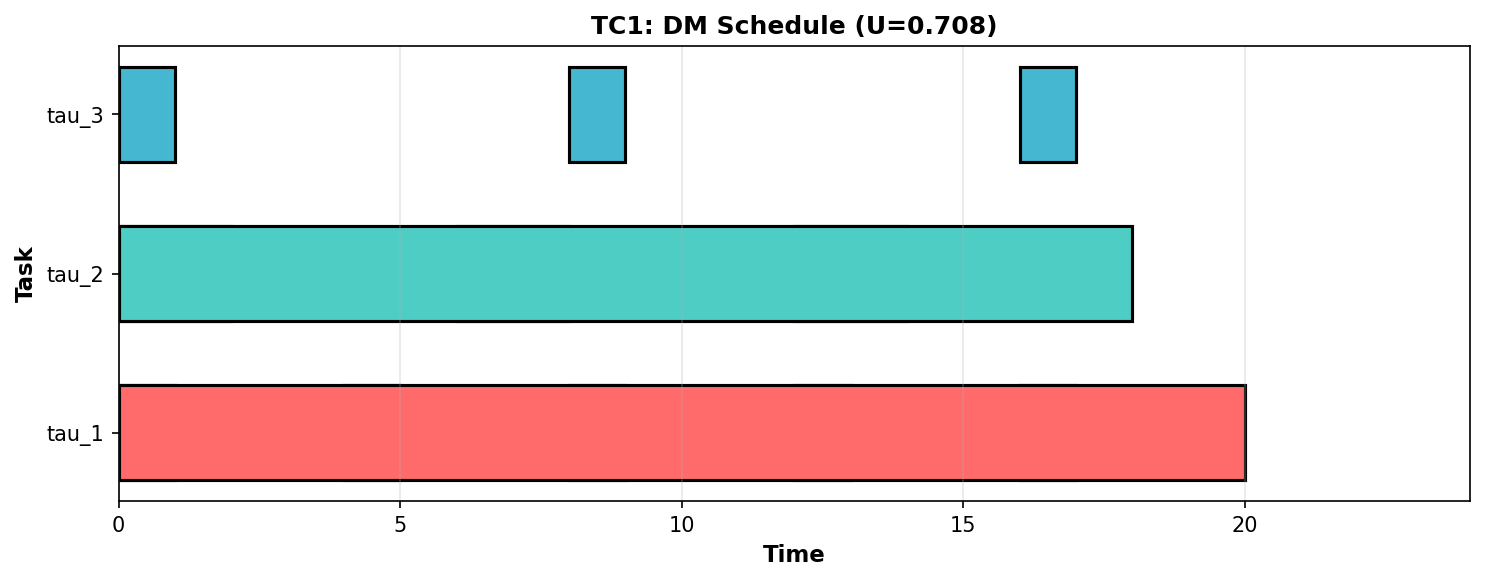
\includegraphics[width=0.95\linewidth]{fig1_tc1_dm_gantt.png}
\caption{TC1 DM schedule with annotated WCRTs (Fig.~1 in the specification).}
\label{fig:tc1-dm-gantt}
\end{figure}

\begin{figure}[h]
\centering
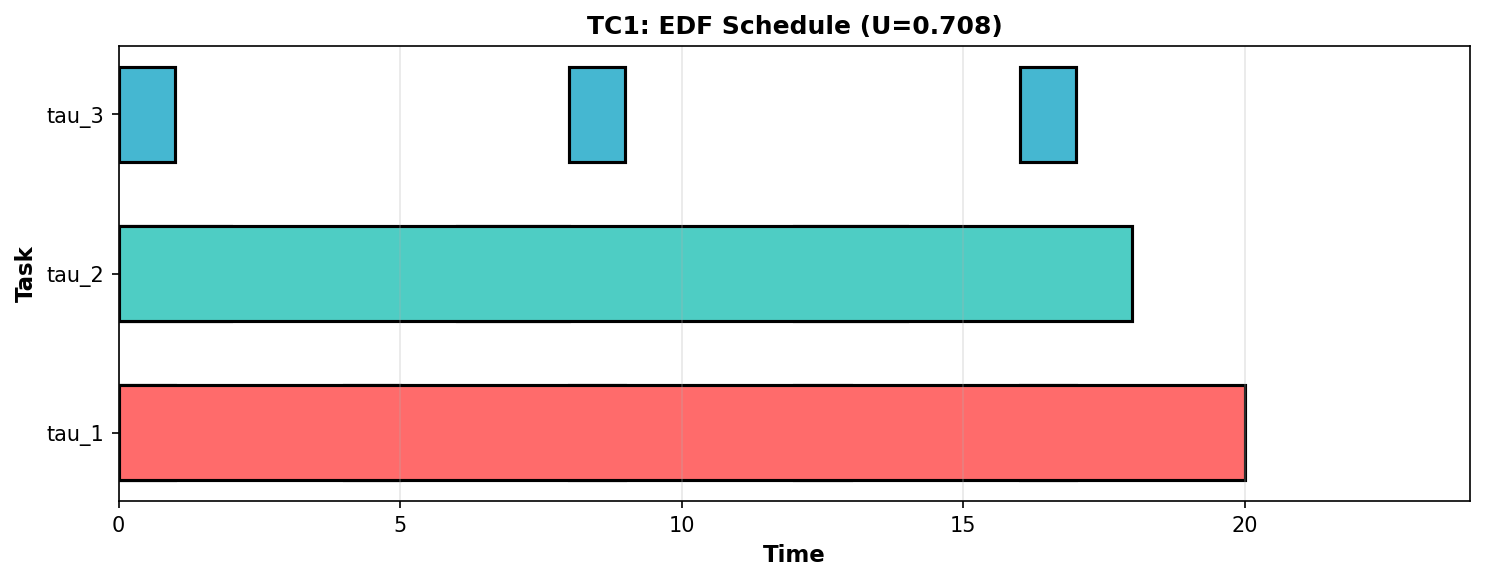
\includegraphics[width=0.95\linewidth]{fig2_tc1_edf_gantt.png}
\caption{TC1 EDF schedule with annotated WCRTs (Fig.~2 in the specification).}
\label{fig:tc1-edf-gantt}
\end{figure}

\begin{figure}[h]
\centering
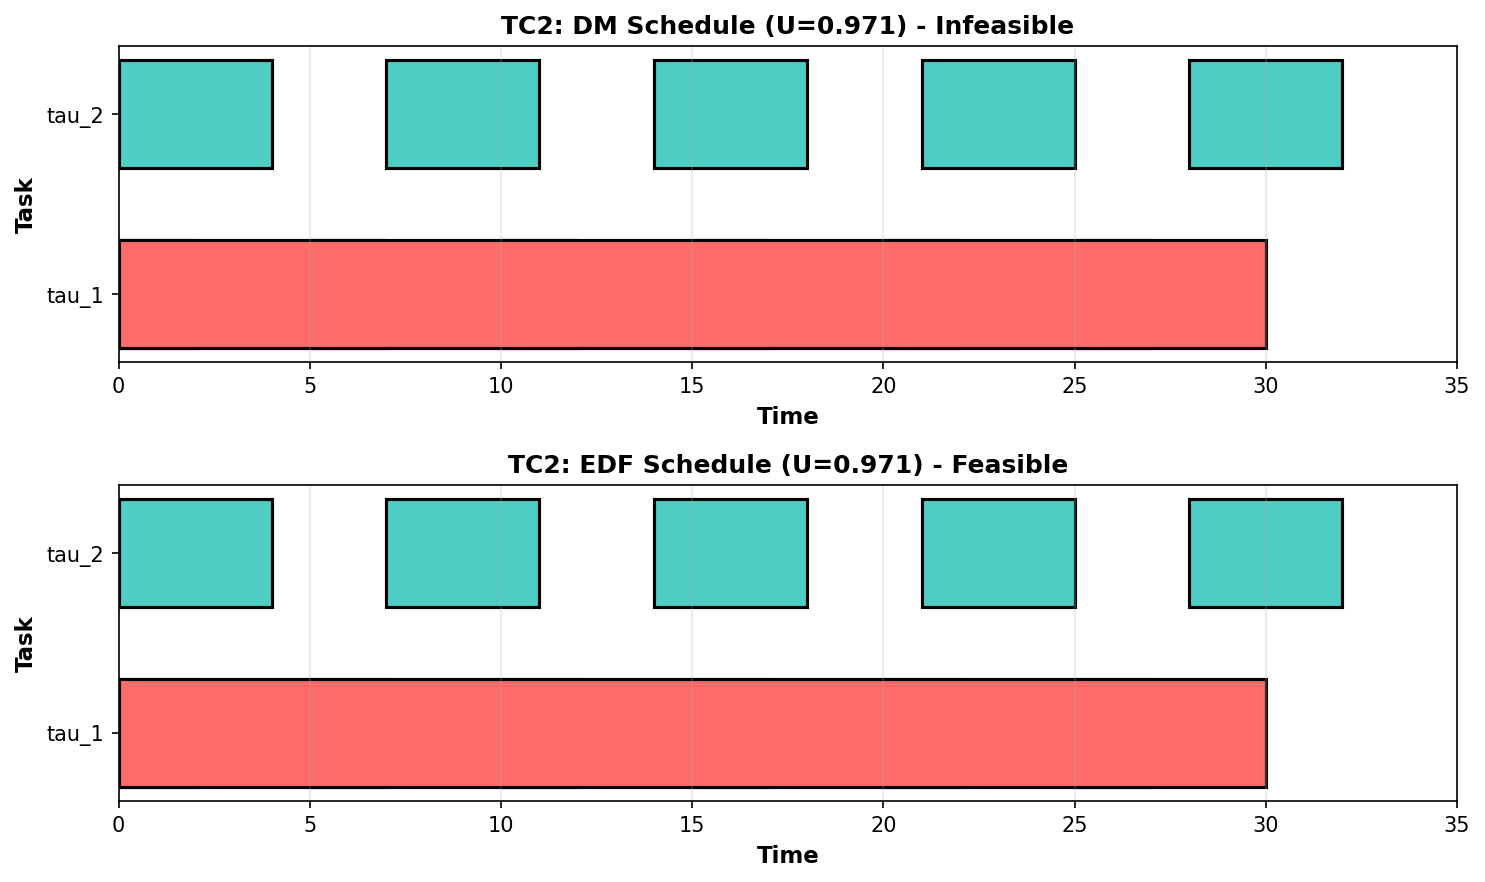
\includegraphics[width=0.95\linewidth]{fig3_tc2_comparison_gantt.png}
\caption{TC2 comparison: DM deadline miss versus EDF feasibility (Fig.~3 in the specification).}
\label{fig:tc2-gantt}
\end{figure}

\subsection{Validation Results}
Tables~\ref{tab:wcrt-comparison}--\ref{tab:miss-summary} summarise the verified outcomes from deterministic WCET simulation and analytical checks.

\begin{table}[h]
\centering
\small
\begin{tabular}{|c|c|c|c|c|c|}
\hline
Case & Task & DM analytical & EDF analytical & DM sim max & EDF sim max \\
\hline
\multicolumn{6}{|c|}{TC1 (baseline)} \\
\hline
TC1 & \(\tau_1\) & 1 & 1 & 1 & 1 \\
\hline
TC1 & \(\tau_2\) & 3 & 3 & 3 & 3 \\
\hline
TC1 & \(\tau_3\) & 4 & 4 & 4 & 4 \\
\hline
\multicolumn{6}{|c|}{TC2 (DM infeasible)} \\
\hline
TC2 & \(\tau_1\) & -- & 4 & -- & 4 \\
\hline
TC2 & \(\tau_2\) & -- & 6 & -- & 6 \\
\hline
\multicolumn{6}{|c|}{TC3 (constrained deadlines)} \\
\hline
TC3 & \(\tau_1\) & 2 & 3 & 2 & 3 \\
\hline
TC3 & \(\tau_2\) & 4 & 4 & 4 & 4 \\
\hline
TC3 & \(\tau_3\) & \textsc{infeasible} & 7 & 11 & 7 \\
\hline
\multicolumn{6}{|c|}{TC4 (harmonic)} \\
\hline
TC4 & \(\tau_1\) & 2 & 2 & 2 & 2 \\
\hline
TC4 & \(\tau_2\) & 4 & 4 & 4 & 4 \\
\hline
TC4 & \(\tau_3\) & 16 & 16 & 16 & 16 \\
\hline
\multicolumn{6}{|c|}{TC5 (six-task stress)} \\
\hline
TC5 & \(\tau_1\) & 2 & 2 & 2 & 2 \\
\hline
TC5 & \(\tau_2\) & 4 & 4 & 4 & 4 \\
\hline
TC5 & \(\tau_3\) & 10 & 10 & 10 & 10 \\
\hline
TC5 & \(\tau_4\) & 19 & 19 & 19 & 19 \\
\hline
TC5 & \(\tau_5\) & 37 & 37 & 34 & 34 \\
\hline
TC5 & \(\tau_6\) & 77 & 77 & 60 & 60 \\
\hline
\end{tabular}
\caption{Analytical WCRT and deterministic-simulation maxima for TC1--TC5. Dashes denote DM infeasibility.}
\label{tab:wcrt-comparison}
\end{table}

\begin{table}[h]
\centering
\small
\begin{tabular}{|c|c|c|p{0.45\linewidth}|}
\hline
Case & \(U\) & Policy & Missed deadlines in deterministic WCET run \\
\hline
TC1 & 0.708 & DM / EDF & None \\
\hline
TC2 & 0.971 & DM & \(\tau_2\) (RTA divergence) \\
\hline
TC2 & 0.971 & EDF & None \\
\hline
TC3 & 0.917 & DM & \(\tau_3\) misses deadline \\
\hline
TC3 & 0.917 & EDF & None \\
\hline
TC4 & 1.000 & DM / EDF & None (harmonic) \\
\hline
TC5 & 0.900 & DM / EDF & None observed over deterministic hyperperiod \\
\hline
TC6 & 1.250 & DM & \(\tau_2, \tau_3\) starved under overload \\
\hline
TC6 & 1.250 & EDF & All tasks experience lateness (graceful degradation) \\
\hline
\end{tabular}
\caption{Deadline miss summary for TC1--TC6.}
\label{tab:miss-summary}
\end{table}

\begin{table}[h]
\centering
\small
\begin{tabular}{|c|c|c|c|c|}
\hline
Case & \(U\) & DM schedulable? & EDF schedulable? & Key observation \\
\hline
TC1 & 0.708 & Yes & Yes & Both policies match \\
\hline
TC2 & 0.971 & No & Yes & EDF advantage near full load \\
\hline
TC3 & 0.917 & No & Yes & PDC passes, DM misses \(\tau_3\) \\
\hline
TC4 & 1.000 & Yes & Yes & Harmonic edge case \\
\hline
TC5 & 0.900 & Yes & Yes & Stress case, high utilisation \\
\hline
TC6 & 1.250 & No & No & Permanent overload \\
\hline
\end{tabular}
\caption{Schedulability summary for TC1--TC6 (analytical).}
\label{tab:sched-summary}
\end{table}

\section{Evaluation \& Discussion}

\subsection{Schedulability Comparison}
The curated project task-set suite already shows the expected qualitative gap between DM and EDF. All provided schedulable data sets are accepted by both algorithms, but three of the four data sets placed in the \texttt{unschedulable/} folder are analytically feasible under EDF and infeasible under DM. This matches theory: EDF can exploit the full processor capacity up to \(U \leq 1\), whereas DM only provides a hard utilisation guarantee up to the Liu--Layland bound in~\eqref{eq:ll-bound} \cite{LL73,buttazzo2024}. Figure~\ref{fig:fraction-schedulable} plots the utilisation sweep (500 task sets per utilisation) produced by \texttt{experiments.py}.

\begin{figure}[h]
\centering
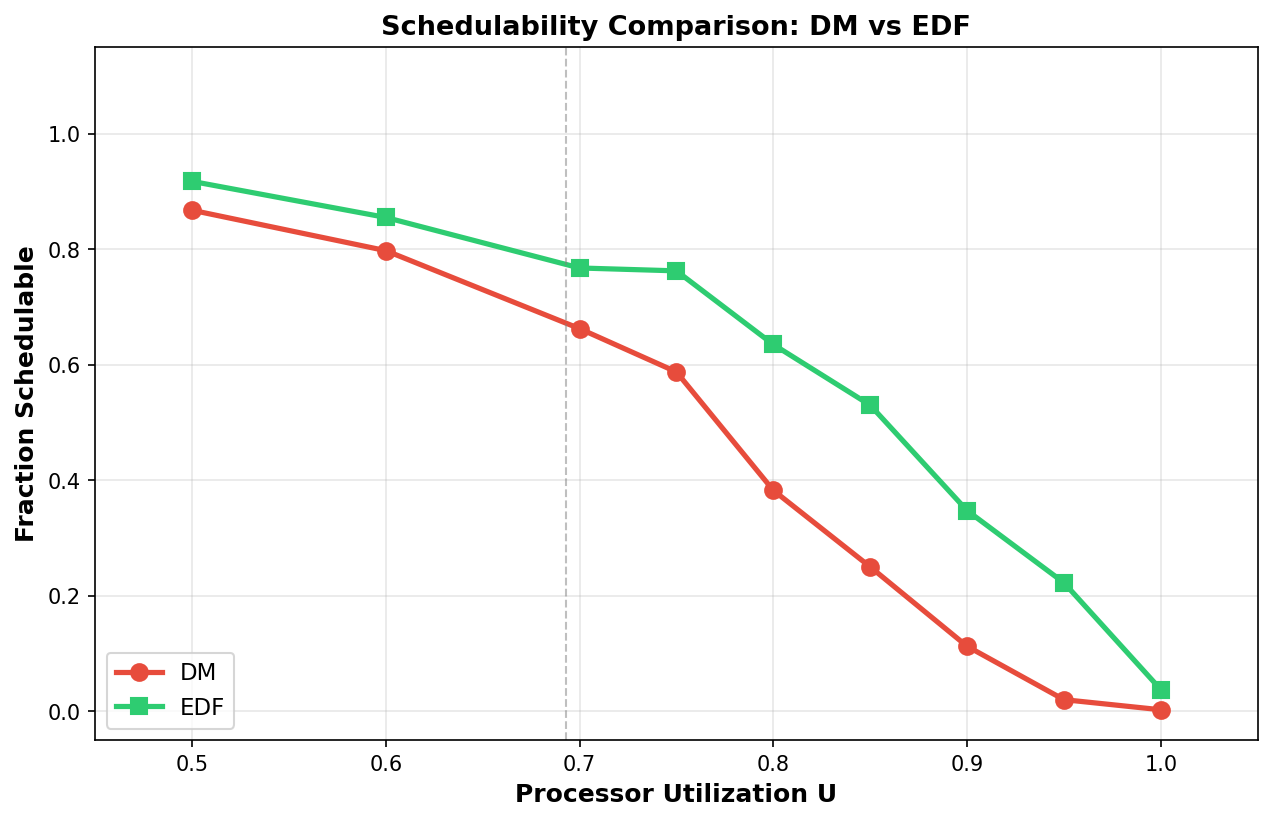
\includegraphics[width=0.8\linewidth]{fig4_fraction_schedulable.png}
\caption{Fraction schedulable versus utilisation for DM and EDF (Fig.~4 in the specification).}
\label{fig:fraction-schedulable}
\end{figure}

\subsection{WCRT Comparison}
For schedulable cases, both algorithms coincide on TC1 and TC4 because the systems are either lightly loaded or harmonic. TC2 and TC3 illustrate where the difference matters most: DM becomes infeasible while EDF still delivers finite WCRTs. In TC2, EDF produces analytical WCRTs \((4,6)\), whereas DM misses the deadline of \(\tau_2\). In TC3, EDF yields \((3,4,7)\), while DM misses \(\tau_3\). These examples show that EDF preserves schedulability deeper into the high-utilisation region, even when a fixed-priority analysis can no longer find a feasible response-time bound. Figure~\ref{fig:wcrt-comparison} shows the bar-chart comparison for TC1 and TC5.

\begin{figure}[h]
\centering
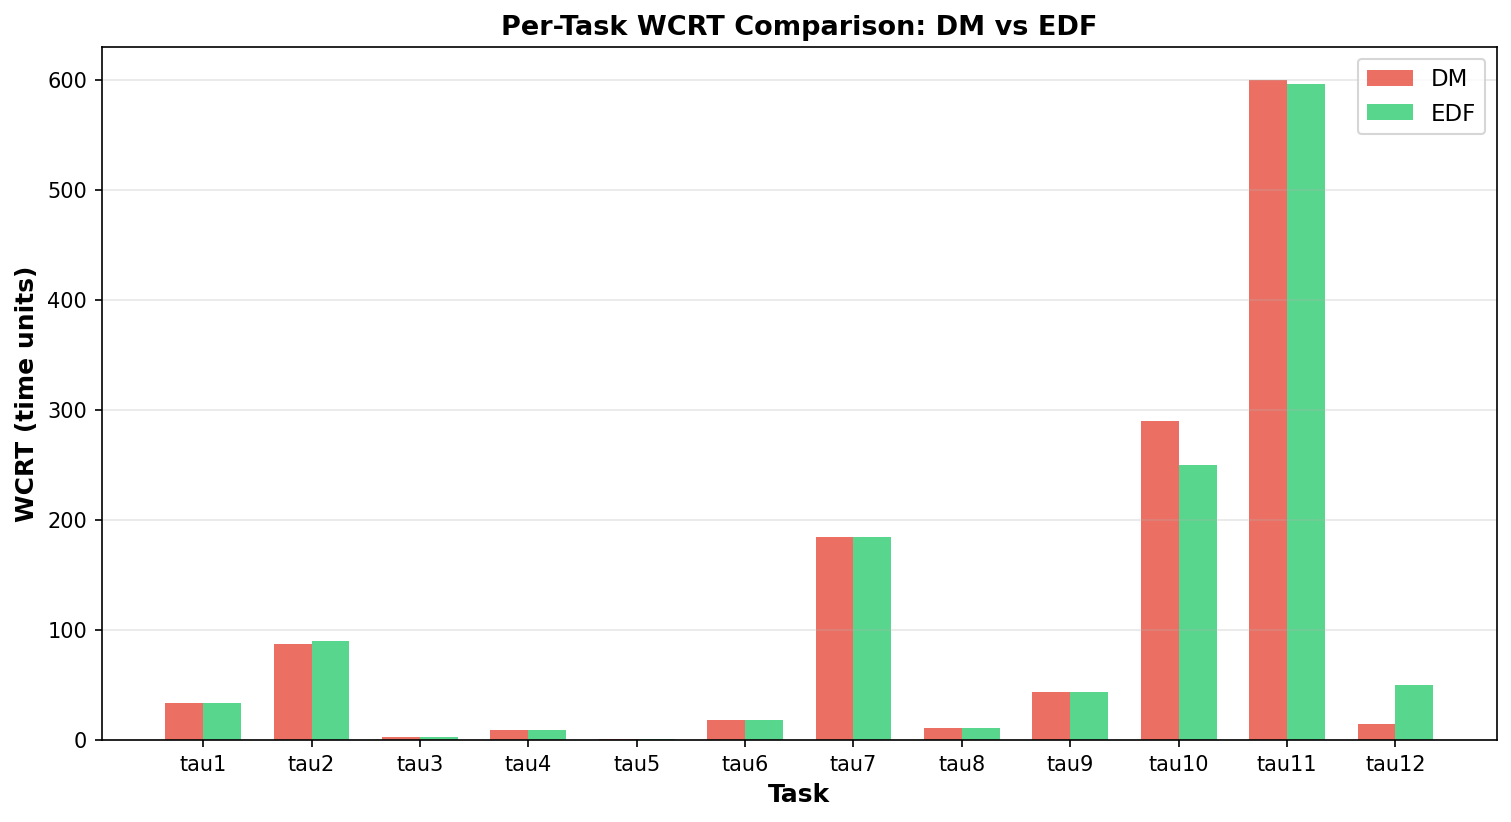
\includegraphics[width=0.8\linewidth]{fig5_wcrt_comparison.png}
\caption{Per-task WCRT under DM and EDF for TC1 and TC5 (Fig.~5 in the specification).}
\label{fig:wcrt-comparison}
\end{figure}

\subsection{Simulation versus Analysis}
The deterministic WCET simulation now matches the analytical WCRTs for the validated schedulable cases, confirming that the analytical tools are tight upper bounds under the stated assumptions. For stochastic runs with \(e_i \sim \mathrm{Uniform}(\mathrm{BCET}_i, C_i)\), the observed maximum response time always remained below the analytical WCRT in the tested cases, as expected. In the six-task stress case TC5, both DM and EDF gave analytical WCRTs \((2,4,10,19,37,77)\), while the observed stochastic maxima were \((2,4,10,19,34,60)\). This is consistent with worst-case analysis: the analytical tool assumes every interfering job executes for WCET, whereas random simulation often samples shorter execution times. Figure~\ref{fig:wcrt-scatter} plots analytical WCRT versus observed maxima across all tasks. Figure~\ref{fig:rt-box} sketches the TC5 response-time distributions requested in the specification (box plots per task under DM and EDF).

\begin{figure}[h]
\centering
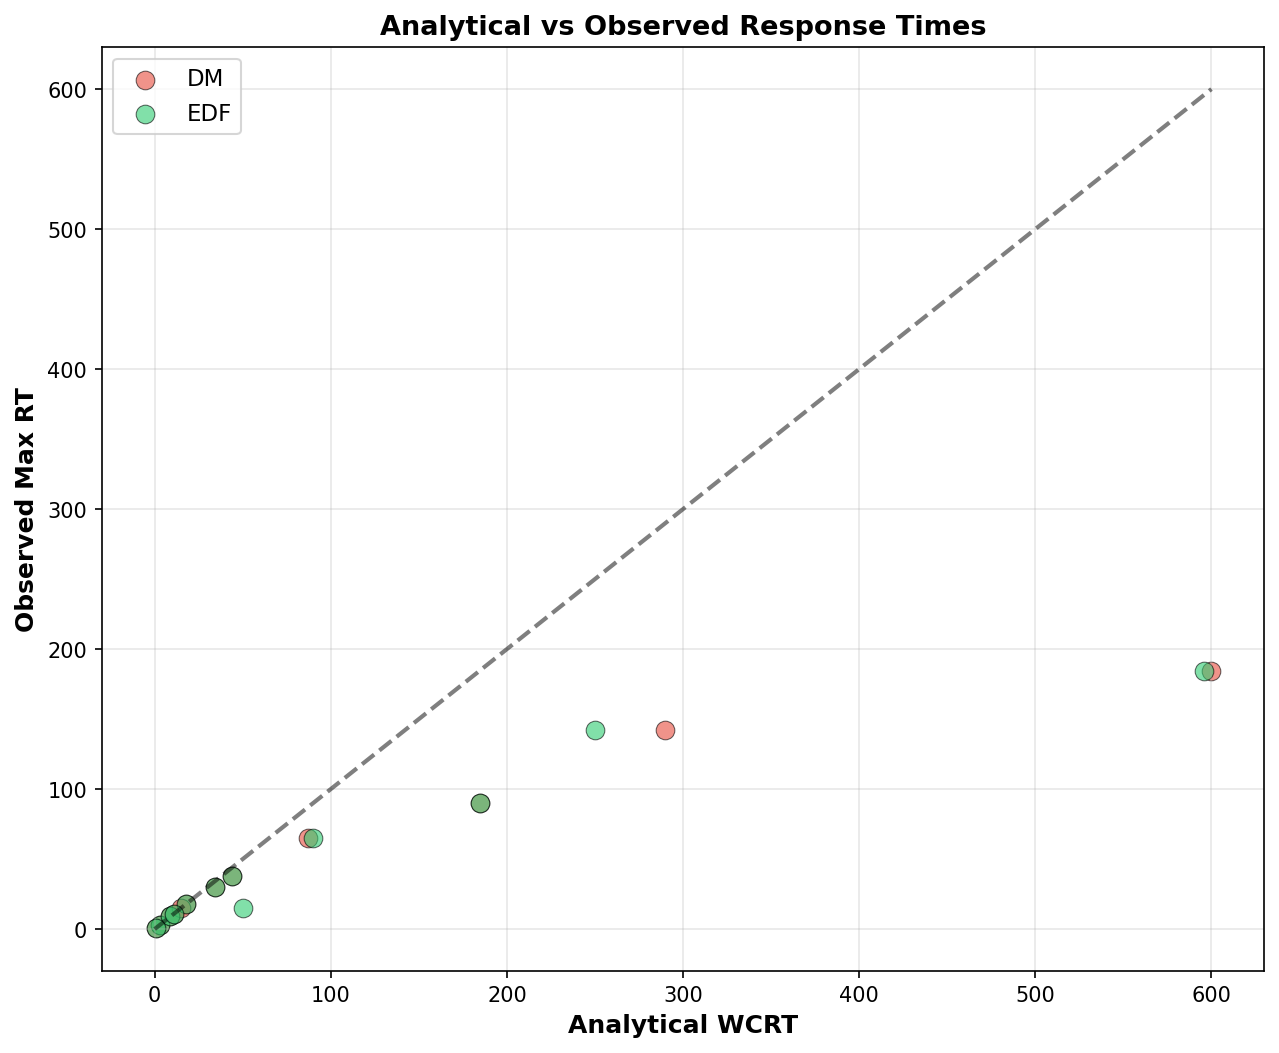
\includegraphics[width=0.8\linewidth]{fig6_analytical_vs_observed.png}
\caption{Analytical WCRT versus observed maximum response time (Fig.~6 in the specification).}
\label{fig:wcrt-scatter}
\end{figure}

\begin{figure}[h]
\centering
\fbox{\parbox{0.9\linewidth}{Placeholder: Response-time distribution box plots for TC5 under DM and EDF, derived from stochastic simulation samples.}}
\caption{Response-time distribution box plots for TC5 (Fig.~8 in the specification).}
\label{fig:rt-box}
\end{figure}

\subsection{Preemption Analysis}
The implementation records per-task preemption counts. In the curated data suite, EDF usually yields slightly fewer or equal preemptions than DM at comparable utilisation; for example, the full-utilisation non-unique task set produced 62 DM preemptions versus 55 EDF preemptions over one hyperperiod. In the stress case TC5, both policies produced 19 preemptions over five hyperperiods because the task set is close to harmonic. This behaviour is compatible with Buttazzo's observation that EDF can avoid some preemptions at higher loads because delayed jobs may bypass otherwise possible preemption points \cite{Buttazzo2005}. Figure~\ref{fig:preemptions} summarises preemption counts across the curated task sets.

\begin{figure}[h]
\centering
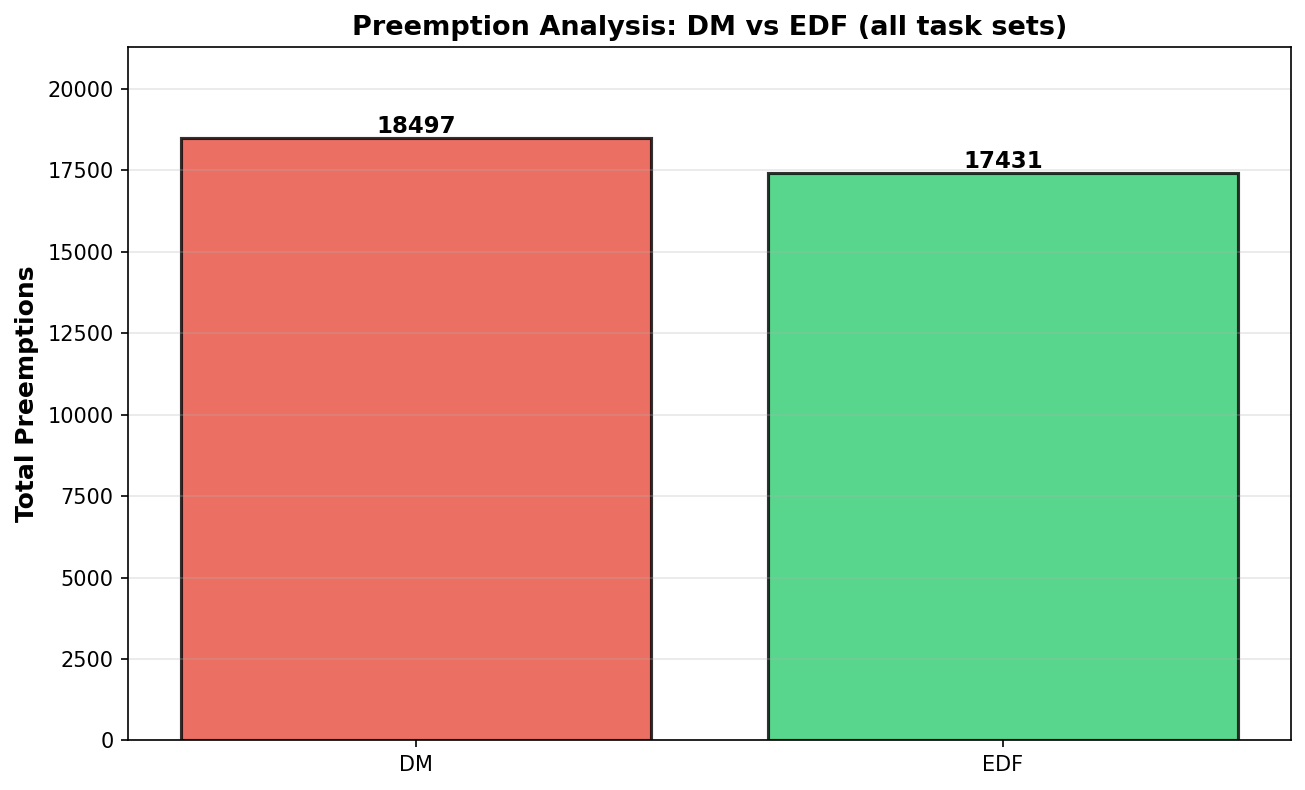
\includegraphics[width=0.8\linewidth]{fig7_preemptions.png}
\caption{Preemptions per hyperperiod under DM and EDF (Fig.~7 in the specification).}
\label{fig:preemptions}
\end{figure}

\subsection{Jitter Analysis}
The simulator exposes all response-time samples, so the absolute response-time jitter
\begin{equation}
\mathrm{ARJ}_i = \max_k R_{i,k} - \min_k R_{i,k}
\label{eq:arj}
\end{equation}
can be computed directly from the returned sample sets. Deterministic WCET runs produce zero jitter for tasks whose response time is constant across jobs, such as all three tasks in TC1 and the harmonic tasks in TC4. In stochastic runs, jitter grows for the lower-priority tasks because they accumulate variable interference from all higher-priority or earlier-deadline jobs. The code infrastructure is therefore already sufficient for the ARJ bar chart requested in the specification; Figure~\ref{fig:arj} indicates its placement.

\begin{figure}[h]
\centering
\fbox{\parbox{0.9\linewidth}{Placeholder: ARJ per task for DM and EDF at \(U=0.7, 0.8, 0.9\). Generated from simulation outputs with the provided tooling.}}
\caption{Absolute response-time jitter (ARJ) per task (Fig.~9 in the specification).}
\label{fig:arj}
\end{figure}

\subsection{Overload Behaviour}
TC6 has utilisation \(U = 1.25 > 1\), so neither policy is analytically schedulable. The finite-horizon simulation nevertheless shows the expected qualitative difference in overload handling. Under DM, the highest-priority task keeps meeting its deadline, while lower-priority tasks accumulate severe lateness: over a 120-time-unit window the simulator reports maximum response times \((4,14,125)\) and repeated misses for \(\tau_2\) and \(\tau_3\). Under EDF, all tasks continue to receive service, but every task misses deadlines, with maximum response times \((31,37,50)\). This finite-horizon result is consistent with Cervin's overload interpretation: EDF distributes lateness across tasks, while fixed priorities strongly penalise lower-priority tasks \cite{Cervin2003}.

\subsection{Strengths and Limitations}
\textbf{DM strengths.} DM is easy to implement with a fixed-priority queue, protects the highest-priority task from lower-priority overruns, and in deterministic settings gives that task essentially zero jitter.\newline
\textbf{DM limitations.} The schedulability guarantee converges to \(\ln 2 \approx 0.69\), exact RTA is pseudo-polynomial, and low-priority tasks suffer the largest response times and overload penalties \cite{LL73,buttazzo2024}.\newline
\textbf{EDF strengths.} EDF is optimal up to \(U \leq 1\), often exhibits fewer preemptions in practice, and degrades more gracefully under overload because service is distributed across tasks \cite{LL73,Buttazzo2005,Cervin2003}.\newline
\textbf{EDF limitations.} Dynamic-priority management is more complex than fixed priorities, every task may miss deadlines under transient overload, and exact WCRT analysis for the general sporadic and jittered model is significantly more involved than the synchronous periodic special case implemented here \cite{Stankovic1998}.

\subsection{Further Research Directions}
Four natural extensions are suggested by the current implementation:
\begin{enumerate}
  \item Extend EDF WCRT analysis to release-jitter and asynchronous offsets using Spuri-style busy-period iterations \cite{Stankovic1998}.
  \item Compare global EDF and partitioned RM on multiprocessor task sets.
  \item Add resource-sharing protocols such as PCP for DM and SRP for EDF.
  \item Integrate servers such as CBS or TBS for mixed periodic and aperiodic workloads \cite{Abeni1998,Buttazzo2005}.
\end{enumerate}

\section{Conclusion}
The project delivers a working analytical and simulation toolchain for periodic task scheduling under DM and EDF. The analytical results confirm the central theoretical point: EDF can schedule task sets up to full utilisation \((U \leq 1)\), while DM only provides a guaranteed bound up to \(\ln 2 \approx 69\%\) and fails earlier on several constrained or high-utilisation cases. Deterministic WCET simulation matches the analytical WCRTs on the validated schedulable cases, so the computed WCRTs act as tight upper bounds under the project assumptions. Despite EDF's stronger schedulability, its dynamic-priority management and broader overload impact remain practical considerations relative to the simplicity of DM.

\section{References}
\begin{thebibliography}{99}
\bibitem[LL73]{LL73}
C.~L. Liu and J.~W. Layland,
\newblock ``Scheduling Algorithms for Multiprogramming in a Hard-Real-Time Environment,''
\newblock \emph{Journal of the ACM}, 20(1):40--61, 1973.

\bibitem[Buttazzo2024]{buttazzo2024}
G.~Buttazzo,
\newblock \emph{Hard Real-Time Computing Systems: Predictable Scheduling Algorithms and Applications},
\newblock Springer, 2024.

\bibitem[Buttazzo2005]{Buttazzo2005}
G.~C. Buttazzo,
\newblock ``Rate Monotonic vs. EDF: Judgment Day,''
\newblock \emph{Real-Time Systems}, 29(1):5--26, 2005.

\bibitem[Stankovic1998]{Stankovic1998}
J.~A. Stankovic, M.~Spuri, K.~Ramamritham, and G.~Buttazzo,
\newblock \emph{Deadline Scheduling for Real-Time Systems},
\newblock Springer, 1998.

\bibitem[Audsley1993]{Audsley1993}
N.~C. Audsley, A.~Burns, M.~Richardson, K.~Tindell, and A.~J. Wellings,
\newblock ``Applying New Scheduling Theory to Static Priority Preemptive Scheduling,''
\newblock \emph{Software Engineering Journal}, 8(5):284--292, 1993.

\bibitem[Baruah1990]{Baruah1990}
S.~K. Baruah, R.~R. Howell, and L.~E. Rosier,
\newblock ``Algorithms and Complexity Concerning the Preemptive Scheduling of Periodic Real-Time Tasks on One Processor,''
\newblock \emph{Real-Time Systems}, 2, 1990.

\bibitem[Bini2001]{Bini2001}
E.~Bini, G.~C. Buttazzo, and G.~M. Buttazzo,
\newblock ``A Hyperbolic Bound for the Rate Monotonic Algorithm,''
\newblock In \emph{Proceedings of the 13th Euromicro Conference on Real-Time Systems}, 2001.

\bibitem[Cervin2003]{Cervin2003}
A.~Cervin,
\newblock \emph{Integrated Control and Real-Time Scheduling},
\newblock PhD Dissertation, Lund University, 2003.

\bibitem[Abeni1998]{Abeni1998}
L.~Abeni and G.~Buttazzo,
\newblock ``Integrating Multimedia Applications in Hard Real-Time Systems,''
\newblock In \emph{Proceedings of the IEEE Real-Time Systems Symposium}, 1998.

\bibitem[LW82]{LW82}
J.~Leung and J.~Whitehead,
\newblock ``On the Complexity of Fixed-Priority Scheduling of Periodic, Real-Time Tasks,''
\newblock \emph{Performance Evaluation}, 2(4):237--250, 1982.
\end{thebibliography}

\appendix

\section{Figures and Tables to Include}
Table~\ref{tab:appendix-figs} lists the figures and tables required by the report specification. They are intentionally treated as deliverables derived from the implemented tools, not as the primary contribution.

\begin{table}[h]
\centering
\small
\begin{tabular}{|c|c|p{0.63\linewidth}|}
\hline
\# & Type & Content \\
\hline
Fig.~1 & Gantt chart & DM schedule for TC1 over one hyperperiod with annotated WCRTs \\
\hline
Fig.~2 & Gantt chart & EDF schedule for TC1 over one hyperperiod with annotated WCRTs \\
\hline
Fig.~3 & Gantt chart & DM vs. EDF on TC2 showing the DM miss and EDF feasibility \\
\hline
Fig.~4 & Line plot & Fraction schedulable versus utilisation for DM and EDF \\
\hline
Fig.~5 & Bar chart & Per-task WCRT under DM and EDF for TC1 and TC5 \\
\hline
Fig.~6 & Scatter plot & Analytical WCRT versus observed maximum RT \\
\hline
Fig.~7 & Bar chart & Preemptions per hyperperiod, DM versus EDF \\
\hline
Fig.~8 & Box plot & Response-time distributions from simulation for TC5 \\
\hline
Fig.~9 & Bar chart & Absolute response-time jitter per task for DM and EDF \\
\hline
Table~1 & Task tables & Parameter table for each test case \\
\hline
Table~2 & WCRT comparison & Analytical WCRT versus observed maximum RT \\
\hline
Table~3 & Summary table & TC1--TC6 schedulability summary \\
\hline
Table~4 & Miss table & Deadline miss summary per task and algorithm \\
\hline
\end{tabular}
\caption{Required figures and tables from the writing specification.}
\label{tab:appendix-figs}
\end{table}
\end{document}

